\documentclass{article}
\usepackage{graphicx} % Required for inserting images

\title{Test 2}
\author{Benjamin Hornacek}
\date{January 2025}

\begin{document}

\maketitle
\section*{Damped Harmonic Oscillator: Overview and Solutions}


A damped harmonic oscillator is a system in which an object experiences both restoring forces, which tend to bring it back to equilibrium, and damping forces, which resist motion and dissipate energy. Such systems are common in physical situations involving oscillations, such as a mass on a spring with friction, or a pendulum in air, where the oscillations gradually decay over time due to energy losses (e.g., through air resistance or internal friction).

\section{Basic Concepts and Setup}

In the simplest form, a harmonic oscillator is a system where the restoring force is proportional to the displacement from equilibrium, as described by Hooke's law. However, in the presence of damping, an additional force is introduced that is proportional to the velocity of the object.

Consider a \textbf{mass} \( \mathbf{m} \) attached to a spring with \textbf{spring constant \( \mathbf{k} \)}, moving on a surface where a \textbf{damping force \( \mathbf{b\dot{x}} \)} (where \( b \) is the damping coefficient) acts opposite to the direction of motion. The total force acting on the mass is a combination of:

- \textbf{Restoring force}: \( -kx \), where \( x \) is the displacement from equilibrium.

- \textbf{Damping force}: \( -b \dot{x} \), where \( \dot{x} \) is the velocity.

The equation of motion for this system can be written as:
\[
m \ddot{x} + b \dot{x} + kx = 0
\]
where:
- \( \ddot{x} \) is the acceleration (second derivative of displacement with respect to time),
- \( \dot{x} \) is the velocity (first derivative of displacement),
- \( x \) is the displacement of the mass from the equilibrium position.

\section{Types of Damping}

The behavior of the system depends on the relative magnitude of the damping coefficient \( b \) and the mass \( m \). There are three main types of damping:

- \textbf{Underdamped}: When \( b^2 < 4mk \), the damping force is small relative to the restoring force, and the system undergoes oscillations that gradually decay over time.\newline

- \textbf{Critically damped}: When \( b^2 = 4mk \), the system returns to equilibrium as quickly as possible without oscillating.\newline

- \textbf{Overdamped}: When \( b^2 > 4mk \), the damping force is so large that the system slowly returns to equilibrium without oscillating.\newline

\section{Equation of Motion} 

The general second-order linear differential equation governing the motion of the damped harmonic oscillator is:

\[
m \ddot{x} + b \dot{x} + kx = 0
\]
This can be simplified by dividing through by \( m \):
\[
\ddot{x} + 2\zeta \omega_0 \dot{x} + \omega_0^2 x = 0
\]
where:

- \( \omega_0 = \sqrt{\frac{k}{m}} \) is the natural frequency of the undamped oscillator,

- \( \zeta = \frac{b}{2\sqrt{mk}} \) is the damping ratio, a dimensionless quantity that characterizes the type of damping.

\section{Solution to the Equation of Motion}

To solve the equation, we first recognize that it is a second-order linear homogeneous differential equation with constant coefficients. The general solution depends on the value of the damping ratio \( \zeta \).


\subsection{Underdamped Case ( \( \zeta < 1 \) )}

For underdamping, the system still oscillates, but with a gradually decreasing amplitude. The solution to the equation is:

\[
x(t) = A e^{-\zeta \omega t} \cos(\omega t + \phi)
\]
where:

- \( A \) is the initial amplitude of oscillation,

- \( \omega\) is the angular frequency,

- \( \phi \)  is the phase angle at \(t = 0\), which depends on the initial conditions.
\newline
This solution describes oscillations with a gradually decaying amplitude over time due to the damping effect.
\newpage
Here is a Graph of this solution:
\begin{center}
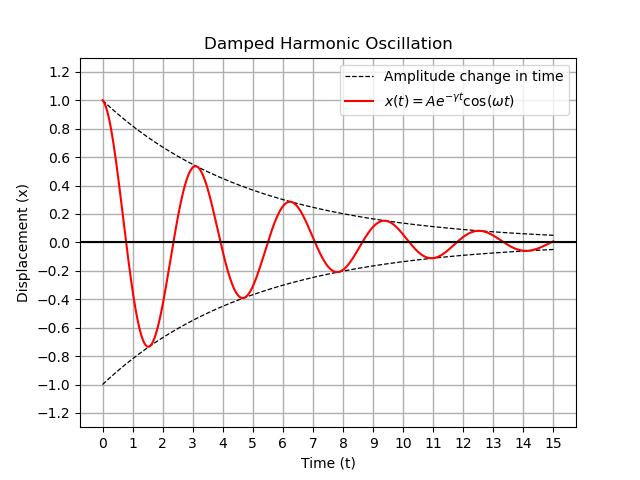
\includegraphics[width= 0.9\linewidth]{Damped_osicllation.png}    
\end{center}

Note two things: \(\gamma\ = \zeta \omega \) is the decay rate which has units of inverse time. The phase angle \(\phi = 0\).
\subsection{Critically Damped and Overdamped Cases}

For the critically damped case (\( \zeta = 1 \)), the solution is:
\[
x(t) = (A + Bt) e^{-\omega t}
\]
This represents a non-oscillatory return to equilibrium, where the object moves as quickly as possible to the equilibrium position without oscillating.
\newline
\newline
For the overdamped case (\( \zeta > 1 \)), the solution is:
\[
x(t) = A e^{r_1 t} + B e^{r_2 t}
\]
where \( r_1 \) and \( r_2 \) are the roots of the characteristic equation \( r^2 + 2\zeta \omega r + \omega^2 = 0 \). These roots are real and distinct, and the solution describes a non-oscillatory motion where the system slowly returns to equilibrium.

\section{Physical Interpretation} 


In the underdamped regime, the system continues to oscillate, but with each cycle, the amplitude of oscillation decreases due to the energy lost as heat or other forms of dissipation through the damping force. This behavior is observed in many physical systems, such as mechanical vibrations in car suspensions or electrical circuits with resistive elements.

In the critically damped case, the system returns to equilibrium as quickly as possible without oscillating, which is desirable in many applications where quick stabilization is needed, such as in clock mechanisms or door closers.

In the overdamped case, the system returns to equilibrium slowly, and no oscillations occur. This behavior can be seen in certain types of mechanical systems with very strong damping, where a quick return to equilibrium is not as important.

\section{Summary}

The damped harmonic oscillator is a fundamental system in physics and engineering, modeling real-world systems where energy dissipation occurs. The equation of motion governing this system is a second-order differential equation, and its solution varies depending on the damping ratio. In the underdamped case, the system oscillates with decreasing amplitude, while in the critically and overdamped cases, the system returns to equilibrium without oscillations. Understanding the behavior of such systems is crucial in designing everything from mechanical systems to electrical circuits and even biological models.

\end{document}
